%%%%%%%%%%%%%%%%%%%%%%%%%%%%%%%%%%%%%%%%%
% Beamer Presentation
% LaTeX Template
% Version 1.0 (10/11/12)
%
% This template has been downloaded from:
% http://www.LaTeXTemplates.com
%
% License:
% CC BY-NC-SA 3.0 (http://creativecommons.org/licenses/by-nc-sa/3.0/)
%
%%%%%%%%%%%%%%%%%%%%%%%%%%%%%%%%%%%%%%%%%

%----------------------------------------------------------------------------------------
%	PACKAGES AND THEMES
%----------------------------------------------------------------------------------------

\documentclass{beamer}

\mode<presentation> {

% The Beamer class comes with a number of default slide themes
% which change the colors and layouts of slides. Below this is a list
% of all the themes, uncomment each in turn to see what they look like.

%\usetheme{default}
%\usetheme{AnnArbor}
%\usetheme{Antibes}
%\usetheme{Bergen}
%\usetheme{Berkeley}
%\usetheme{Berlin}
%\usetheme{Boadilla}
%\usetheme{CambridgeUS}
%\usetheme{Copenhagen}
%\usetheme{Darmstadt}
%\usetheme{Dresden}
%\usetheme{Frankfurt}
%\usetheme{Goettingen}
%\usetheme{Hannover}
%\usetheme{Ilmenau}
%\usetheme{JuanLesPins}
%\usetheme{Luebeck}
\usetheme{Madrid}
%\usetheme{Malmoe}
%\usetheme{Marburg}
%\usetheme{Montpellier}
%\usetheme{PaloAlto}
%\usetheme{Pittsburgh}
%\usetheme{Rochester}
%\usetheme{Singapore}
%\usetheme{Szeged}
%\usetheme{Warsaw}

% As well as themes, the Beamer class has a number of color themes
% for any slide theme. Uncomment each of these in turn to see how it
% changes the colors of your current slide theme.

%\usecolortheme{albatross}
%\usecolortheme{beaver}
%\usecolortheme{beetle}
%\usecolortheme{crane}
%\usecolortheme{dolphin}
%\usecolortheme{dove}
%\usecolortheme{fly}
%\usecolortheme{lily}
\usecolortheme{orchid}
%\usecolortheme{rose}
%\usecolortheme{seagull}
%\usecolortheme{seahorse}
%\usecolortheme{whale}
%\usecolortheme{wolverine}

%\setbeamertemplate{footline} % To remove the footer line in all slides uncomment this line
%\setbeamertemplate{footline}[page number] % To replace the footer line in all slides with a simple slide count uncomment this line

%\setbeamertemplate{navigation symbols}{} % To remove the navigation symbols from the bottom of all slides uncomment this line
}

\setbeamertemplate{itemize items}[default]
\setbeamertemplate{enumerate items}[default]

\usepackage{graphicx} % Allows including images
\usepackage{booktabs} % Allows the use of \toprule, \midrule and \bottomrule in tables
\usepackage{tikz}

%----------------------------------------------------------------------------------------
%	TITLE PAGE
%----------------------------------------------------------------------------------------

\title[Short title]{Learning Rules With Categorical Attributes from Linked Data Sources} % The short title appears at
%the bottom of every slide, the full title is only on the title page

\author{Andre de Oliveira Melo} % Your name
\institute[Saarland University] % Your institution as it will appear on the bottom of every slide, may be shorthand to
%save space
{
Saarland University \\ % Your institution for the title page
\medskip
\textit{andresony@gmail.com} % Your email address
}
\date{\today} % Date, can be changed to a custom date

\begin{document}

\begin{frame}
\titlepage % Print the title page as the first slide
\end{frame}

\begin{frame}
\frametitle{Overview} % Table of contents slide, comment this block out to remove it
\tableofcontents % Throughout your presentation, if you choose to use \section{} and \subsection{} commands, these will automatically be printed on this slide as an overview of your presentation
\end{frame}

%----------------------------------------------------------------------------------------
%	PRESENTATION SLIDES
%----------------------------------------------------------------------------------------

%------------------------------------------------
\section{Introduction}
%------------------------------------------------

\subsection{Subsection Example}

\begin{frame}
\frametitle{Semantic Web}
\begin{quote}
 ``provides a common framework that allows data to be shared and reused across application, enterprise, and community
boundaries''
\end{quote}

Built on W3C's:
\begin{itemize}
 \item RDF
 \item OWL
 \item SKOS
 \item SPARQL
\end{itemize}
\end{frame}

%------------------------------------------------

\begin{frame}
\frametitle{Linked Data}
\begin{quote}
 ``a term used to describe a recommended best practises for exposing, sharing, and connecting pieces of data,
information and knowledge on the Semantic Web using URIs and RDF''
\end{quote}
\begin{quote}
 ``collection of interrelated datasets on the Web''
\end{quote}
\end{frame}

%------------------------------------------------

\begin{frame}
\frametitle{Linked Data}
 \begin{figure}
 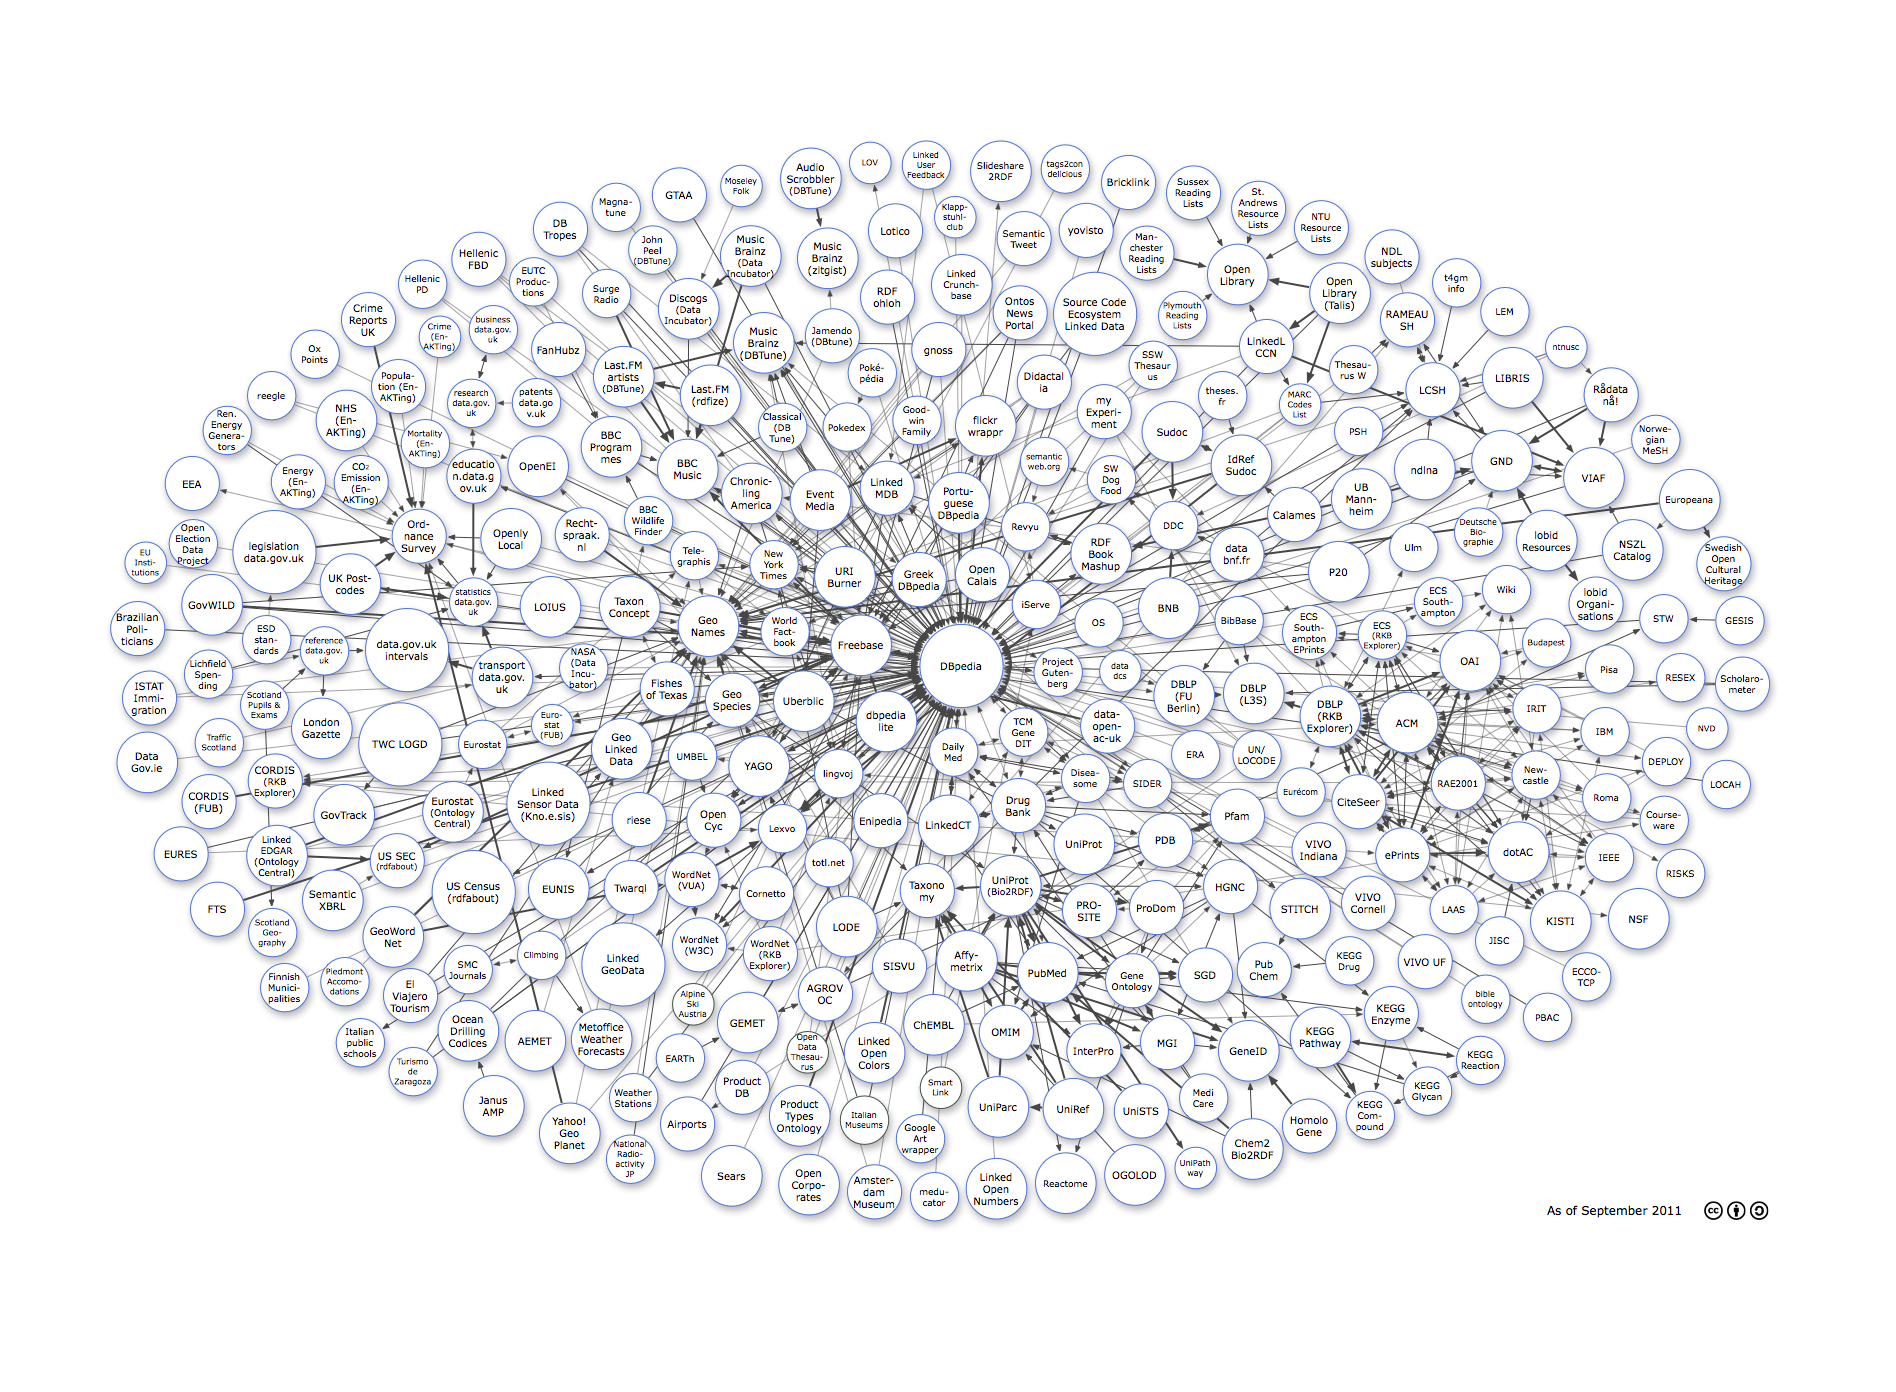
\includegraphics[width=0.8\linewidth]{./Figures/lod-datasets_2011-09-19}
 \end{figure}
\end{frame}

\subsection{Motivation}

\begin{frame}
\frametitle{Motivation}
Learn inference rules from data:
\begin{center}
  $\underbrace{livesIn(x,y)}_{head}$:-$\underbrace{isMarriedTo(x,z),livesIn(z,y)}_{body}$
\end{center}
Support and confidence thresholds
\begin{itemize}
 \item Support: $supp(head$:-$body)=supp(head \cup body)$
 \item Confidence: $conf(head$:-$body)=\cfrac{supp(head \cup body)}{supp(body)}$ 
\end{itemize}
\end{frame}

\begin{frame}
\frametitle{Motivation}
Introducing constants can be relevant, e.g.:
\begin{center}
  \emph{speaks(x,y) :- livesIn(x,z)}\\
  \emph{speaks(x,Portuguese) :- livesIn(x,Brazil)}
\end{center}
What about numerical attributes?
\begin{center}
  \emph{hasChild(x,y) :- hasAge(x,a)} [base-rule]
\end{center}
\begin{itemize}
 \item \textbf{Support}: number of supporting examples
  $supp(head$:-$body)=supp(head \cup body)$
 \item \textbf{Confidence}: $conf(head$:-$body)=\cfrac{supp(head \cup body)}{supp(body)}$ 
\end{itemize}
\end{frame}

\begin{frame}
\frametitle{Motivation}
 We are more interested in base-rules that:
 \begin{itemize}
  \item Satisfy support threshold
  \item Do not satisfy confidence threshold
  \item Potentially has a refined-rule with an interval that satisfies both thresholds \\
    \quad i.e., has non-uniform confidence distribution \\
    \quad i.e., has divergent positive examples and body support distributions
 \end{itemize}
\end{frame}

\begin{frame}
\frametitle{Motivation}
 Problem?
 \begin{itemize}
    \item Search space grows dramatically
    \item Usually unfeasible to perform exhaustive search
    \item Querying support and confidence distributions is very expensive
 \end{itemize}
\end{frame}

\section{Related Work}

\begin{frame}
\frametitle{ILP}
 Inductive Logic Programming: Finds a hypothesis $H$ that covers all positive, and no negative examples
  \begin{equation}
   positiveExamples + negativeExamples + background Knowledge \rightarrow hypothesis
  \end{equation}

\begin{table}
\begin{tabular}{| l | l |}
\toprule
\textbf{Training Examples} & \textbf{Background Knowledge}\\
\midrule
daughter(mary,ann) +	& parent(ann,mary)	\\
daughter(eve,tom) +	& parent(ann, tom)	\\
daughter(tom,ann) - 	& parent(tom,eve)	\\
daughter(eve,ann) -	& parent(tom,ian) 	\\
			& female(ann)		\\
			& female(mary)		\\
			& female(eve)		\\
\bottomrule
\end{tabular}
\end{table}
\end{frame}

\begin{frame}
\frametitle{ILP}
Important concepts:
  \begin{itemize}
   \item Literal: predicate symbol with bracketed n-tuple, e.g: \\ \quad $L=livesIn(x,y)$
   \item Clause: a set of literals (negated or not), e.g: \\ \quad $c=\{L_1,L_2,\ldots,\neg L_{m-1}, \neg L_{m}\}$
   \item Horn Clause: a clause with a single non-negated literal, e.g: \\ \quad$\{L_1,L_2,\neg L_3\} \equiv
L_3$:-$L1,L2$
   \item Hypothesis: a set of clauses $H$
   \item Completeness: $H$ covers all positive examples
   \item Consistency: $H$ covers no negative examples
  \end{itemize}
\end{frame}

\begin{frame}
\frametitle{ILP}
Approaches
  \begin{itemize}
   \item Bottom-up: Start with least general H then perform generalizations
   \item Top-down: Start with most general H then perform specializations
   \begin{itemize}
    \item Specialization loop: adds literals to a clause and ensures consistency
    \item Covering loop: adds clauses to the hypothesis and ensures completeness
   \end{itemize}
  \end{itemize}
\end{frame}

\section{Learning Rules With Categorical Attributes}

\begin{frame}
\frametitle{Correlation between Literals}
Let's say we want to refine a clause with $hasIncome(x,y)$ with an interval for $y$.
What property is more interesting to add to the clause body: 
  \begin{center}
   $quarterOfBirth(x,z)$ or $hasEducation(x,z)$?
  \end{center}
\begin{columns}[c]
  \column{0.5\textwidth}
    \center{quarterOfBirth}
    \begin{figure}
    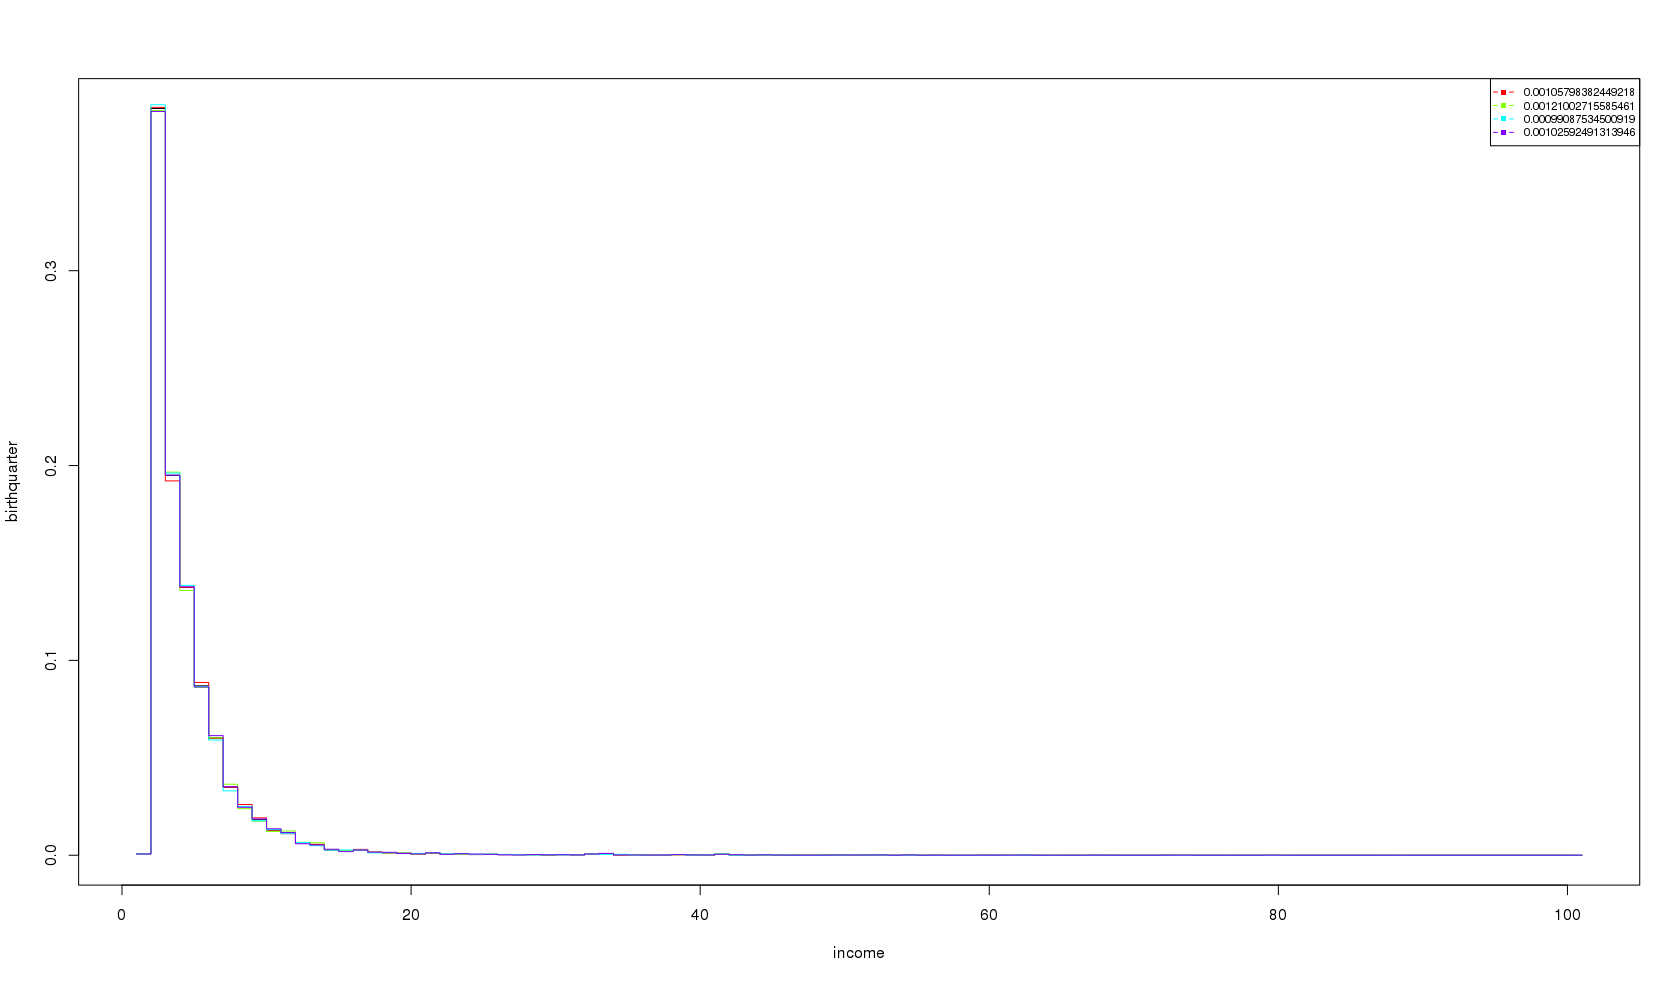
\includegraphics[width=1\linewidth]{./Figures/income-birthquarter.png}
    \end{figure}
  \column{0.5\textwidth}
    \center{hasEducation}
    \begin{figure}
    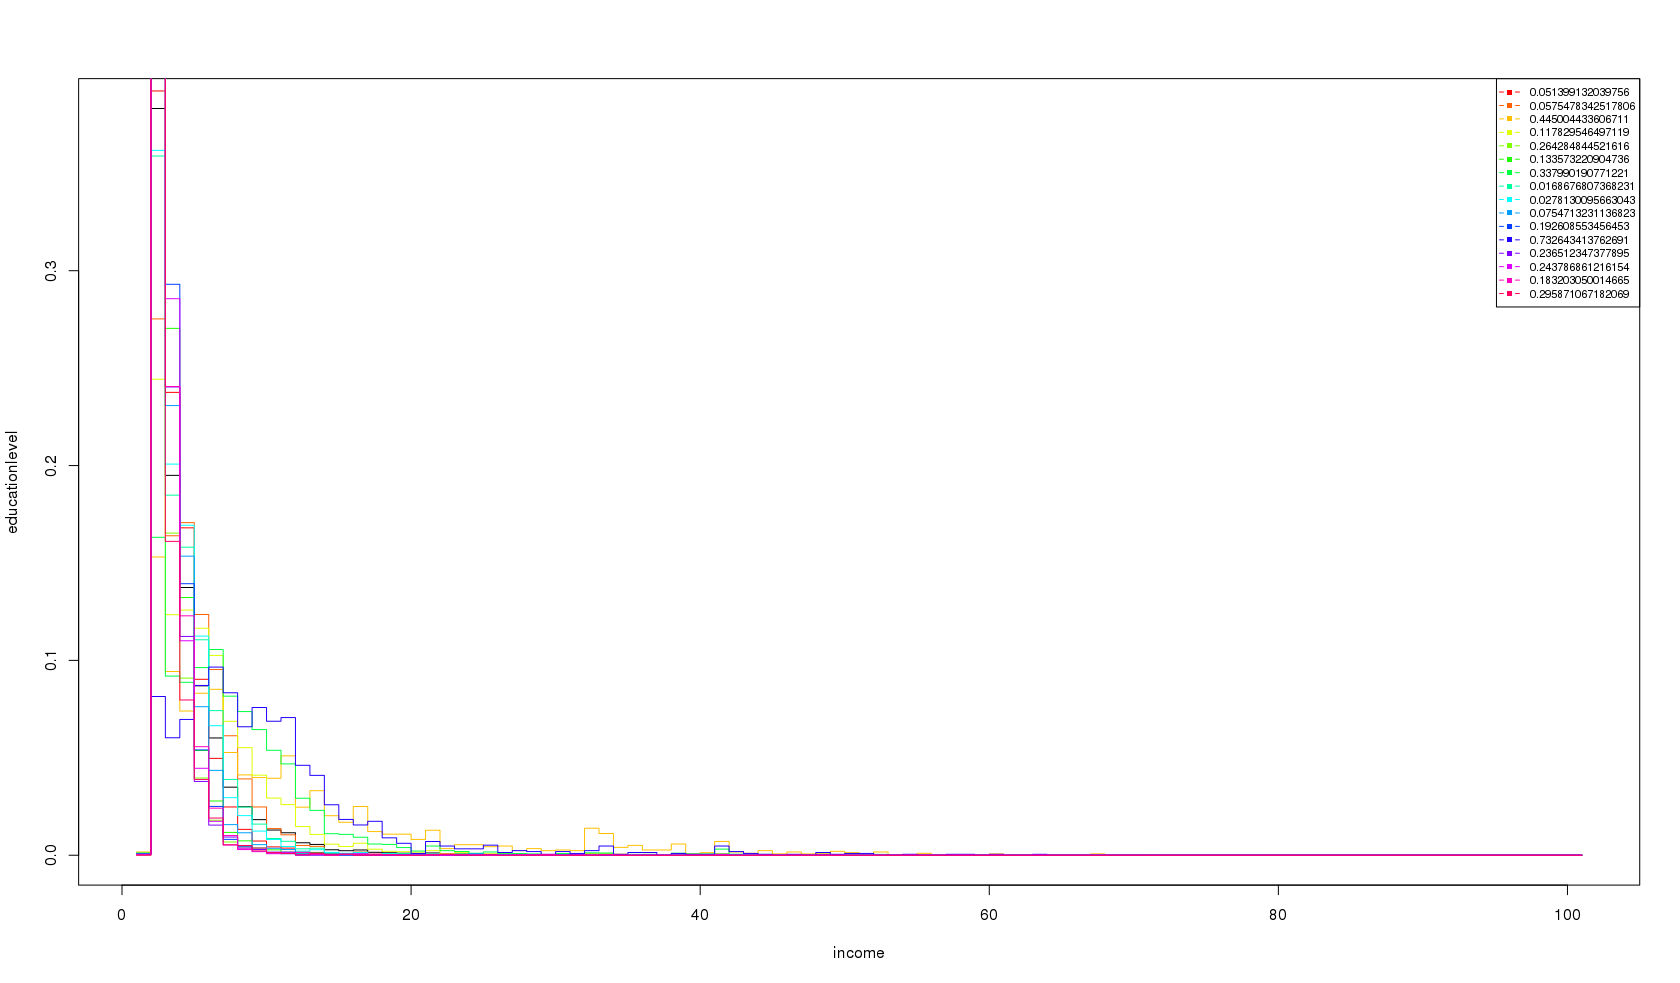
\includegraphics[width=1\linewidth]{./Figures/income-education.png}
    \end{figure}
\end{columns}
\end{frame}

\begin{frame}
\frametitle{Correlation between Literals}
  \begin{figure}
  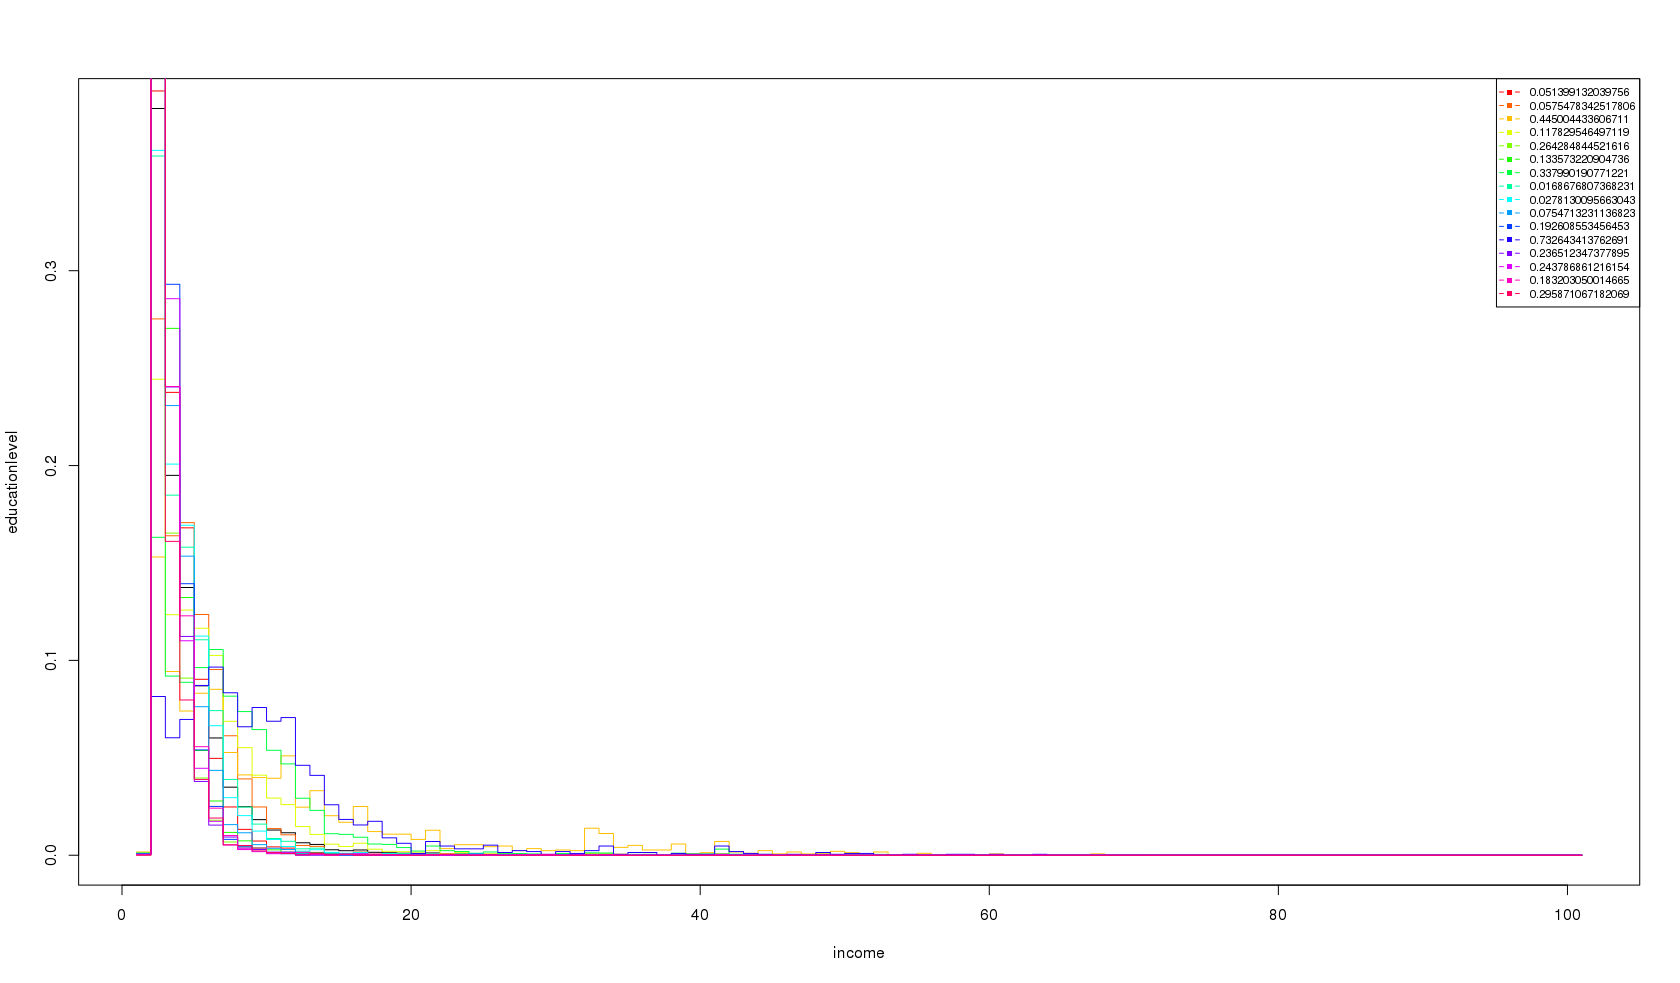
\includegraphics[width=1\linewidth]{./Figures/income-education.png}
  \end{figure}
\end{frame}

\begin{frame}
\frametitle{Correlation between Literals}
  \begin{table} 
    \begin{tabular}{c}
      USCensus constants for $z$ in $hasEducation(x,z)$\\
     \end{tabular}
     \begin{tabular}{l  l}
      \midrule
      N/A (less than 3 years old)	& High school graduate	\\
      No school completed		& Some college, less than 1 year\\
      Nursery school to grade 4   	& One or more years of college, no degree\\
      Grade 5 or grade 6		& Associate's degree\\
      Grade 7 or grade 8		& Bachelor's degree\\
      Grade 9				& Master's degree\\
      Grade 10                   	& Professional school degree\\
      Grade 11				& Doctorate degree\\  
      Grade 12 no diploma   		& \\
    \end{tabular}
  \end{table}
\end{frame}

\begin{frame}
\frametitle{Correlation between Literals}
  Use distribution divergence as interestingness measures, e.g.:
  \quad Kullback-Leibler, Chi-square, Jensen-Shannon, etc. \\
  But, divergence alone isn't a good idea because:
  \begin{itemize}
   \item Lower support histograms are more likely to have a divergent distribution
   \item Still, support is a good measure as well
  \end{itemize}
  Then combine both measures: divergence*support
\end{frame}

\begin{frame}
\frametitle{Correlation Lattice}
  \begin{itemize}
   \item Build a lattice similar to an itemset lattice 
   \item Numerical property as root 
   \item The ``items'' would be literals that can be joined with the root's non-numerical variable 
   \item Each node consists of the joined with a set of literals \\
  Each node has a frequency histogram with examples distribution over root's numerical attribute to enable divergence 
  measures 
   \item Then we can use it to suggest the most interesting literals to be added in the refinement step from core-ILP
   \item Idea is to generate a correlation lattice for each numerical attribute as preprocessing step 
  \end{itemize}
\end{frame}

\begin{frame}
 \frametitle{Correlation Lattice}
\begin{figure}[!h]
  \caption{Correlation Lattice example}
  \centering
  \begin{tikzpicture}
  [scale=0.8,auto=center,every node/.style={circle,fill=black!10,minimum size=1.2cm, font=\tiny}]
  \begin{tikzpicture}
 [scale=1.8,auto=center,every node/.style={minimum, font=\tiny}]
  \node (n0) at (4,10) {$r$};
  \node (na) at (0,8)  {$r a$};
  \node (na1)%[fill=blue!20] 
  at (1,7.5)  {$r a_1$};
  \node (na2)%[fill=blue!20] 
  at (2,7.5) {$r a_2$};
  \node (nb) at (3,8)  {$r b$};
  \node (nb1)%[fill=red!20] 
  at (4,7.5)  {$r b_1$};
  \node (nb2)%[fill=red!20] 
  at (5,7.5)  {$r b_1$};
  \node (nc) at (6,8)  {$r c$};
  \node (nc1)%[fill=green!20] 
  at (7,7.5)  {$r c_1$};
  \node (nc2)%[fill=green!20] 
  at (8,7.5)  {$r c_1$};
  \node (nab) at (0,5)  {$r a b$};
  \node (na1b1)%[fill=magenta!20] 
  at (0.5,4.5)  {$r a_1 b_1$};
  \node (na1b2)%[fill=magenta!20] 
  at (1.0,4.5)  {$r a_1 b_2$};
  \node (na2b1)%[fill=magenta!20] 
  at (1.5,4.5)  {$r a_2 b_1$};
  \node (na2b2)%[fill=magenta!20] 
  at (2.0,4.5)  {$r a_2 b_2$};
  \node (nac) at (3,5)  {$r a c$};
  \node (na1c1)%[fill=cyan!20] 
  at (3.5,4.5)  {$r a_1 c_1$};
  \node (na1c2)%[fill=cyan!20] 
  at (4.0,4.5)  {$r a_1 c_2$};
  \node (na2c1)%[fill=cyan!20] 
  at (4.5,4.5)  {$r a_2 c_1$};
  \node (na2c2)%[fill=cyan!20] 
  at (5.0,4.5)  {$r a_2 c_2$};
  \node (nbc) at (6,5)  {$r b c$};
  \node (nb1c1)%[fill=yellow!50] 
  at (6.5,4.5)  {$r b_1 c_1$};
  \node (nb1c2)%[fill=yellow!50] 
  at (7.0,4.5)  {$r b_1 c_2$};
  \node (nb2c1)%[fill=yellow!50] 
  at (7.5,4.5)  {$r b_2 c_1$};
  \node (nb2c2)%[fill=yellow!50] 
  at (8.0,4.5)  {$r b_2 c_2$};
  \node (nabc) at (2,2)  {$r a b c$};
  \node (na1b1c1)%[fill=black!10] 
  at (2.5,1.5)  {$r a_1 b_1 c_1$};
  \node (na1b1c2)%[fill=black!10] 
  at (3.2,1.5)  {$r a_1 b_1 c_2$};
  \node (na1b2c1)%[fill=black!10] 
  at (3.9,1.5)  {$r a_1 b_2 c_1$};  
  \node (na1b2c2)%[fill=black!10] 
  at (4.6,1.5)  {$r a_1 b_2 c_2$};
  \node (na2b1c1)%[fill=black!10] 
  at (5.3,1.5)  {$r a_2 b_1 c_1$};
  \node (na2b1c2)%[fill=black!10] 
  at (6.0,1.5)  {$r a_2 b_1 c_2$};
  \node (na2b2c1)%[fill=black!10] 
  at (6.7,1.5)  {$r a_2 b_2 c_1$};
  \node (na2b2c2)%[fill=black!10] 
  at (7.4,1.5)  {$r a_2 b_2 c_2$};

  \foreach \from/\to in {na/na1,na/na2,nb/nb1,nb/nb2,nc/nc1,nc/nc2}
    \draw[dashed] (\from) -| (\to);

  \foreach \from/\to in {nab/na1b1,nab/na1b2,nab/na2b1,nab/na2b2}
    \draw[dashed] (\from) -| (\to);

  \foreach \from/\to in {nabc/na1b1c1,nabc/na1b1c2,nabc/na1b2c1,nabc/na1b2c2,nabc/na2b1c1,nabc/na2b1c2,nabc/na2b2c1,nabc/na2b2c2}
    \draw[dashed] (\from) -| (\to);

  \foreach \from/\to in {n0/na1,n0/na2,na1/na1b1,na1/na1b2,na2/na2b1,na2/na2b2,na1/na1c1,na1/na1c2,na2/na2c1,na2/na2c2}
    \draw[blue] (\from) -- (\to);
  \foreach \from/\to in {n0/nb1,n0/nb2,nb1/na1b1,nb1/na2b1,nb2/na1b2,nb2/na2b2,nb1/nb1c1,nb1/nb1c2,nb2/nb2c1,nb2/nb2c2}
    \draw[red] (\from) -- (\to);
  \foreach \from/\to in {n0/nc1,n0/nc2,nc1/na1c1,nc1/na2c1,nc2/na1c2,nc2/na2c2,nc1/nb1c1,nc1/nb2c1,nc2/nb1c2,nc2/nb2c2}
    \draw[green] (\from) -- (\to);
  \foreach \from/\to in {na1b1/na1b1c1,na1b2/na1b2c1,na2b1/na2b1c1,na2b2/na2b2c1,na1b1/na1b1c2,na1b2/na1b2c2,na2b1/na2b1c2,na2b2/na2b2c2}
    \draw[magenta] (\from) -- (\to);
  \foreach \from/\to in {na1c1/na1b1c1,na1c1/na1b2c1,na2c1/na2b1c1,na2c1/na2b2c1,na1c2/na1b1c2,na1c2/na1b2c2,na2c2/na2b1c2,na2c2/na2b2c2}
    \draw[cyan] (\from) -- (\to);
  \foreach \from/\to in {nb1c1/na1b1c1,nb2c1/na1b2c1,nb1c1/na2b1c1,nb2c1/na2b2c1,nb1c2/na1b1c2,nb2c2/na1b2c2,nb1c2/na2b1c2,nb2c2/na2b2c2}
    \draw[yellow] (\from) -- (\to);

  \foreach \from/\to in {n0/na,n0/nb,n0/nc}
    \draw[dashed] (\from) -- (\to);
  \foreach \from/\to in {na/nab,na/nac,nb/nab,nb/nbc,nc/nac,nc/nbc,nab/nabc,nac/nabc,nbc/nabc}
    \draw[dashed] (\from) -- (\to);  
\end{tikzpicture}

  \end{tikzpicture}
  \label{fig:lattice}
\end{figure}
\end{frame}


\begin{frame}
\frametitle{Correlation Lattice}
  \begin{itemize}
     \item Number of nodes in a lattice with $l$ levels $n$ properties and $m$ constants per property:
      \begin{equation}
	\sum_{i=1}^l \dbinom{nm}{i}
      \end{equation}
      \item Too expensive, we need to reduce size 
      \begin{itemize}
	\item prune by support (safe)
      \end{itemize}
      \item If not sufficient, we can restrict the literals to be added in the lattice in order to reduce $n$ and $m$
as much as possible
  \end{itemize}
\end{frame}

%------------------------------------------------

\begin{frame}
\frametitle{Multiple Columns}
\begin{columns}[c] % The "c" option specifies centered vertical alignment while the "t" option is used for top vertical alignment

\column{.45\textwidth} % Left column and width
\textbf{Heading}
\begin{enumerate}
\item Statement
\item Explanation
\item Example
\end{enumerate}

\column{.5\textwidth} % Right column and width
Lorem ipsum dolor sit amet, consectetur adipiscing elit. Integer lectus nisl, ultricies in feugiat rutrum, porttitor sit amet augue. Aliquam ut tortor mauris. Sed volutpat ante purus, quis accumsan dolor.

\end{columns}
\end{frame}

%------------------------------------------------
\section{Second Section}
%------------------------------------------------

\begin{frame}
\frametitle{Table}
\begin{table}
\begin{tabular}{l l l}
\toprule
\textbf{Treatments} & \textbf{Response 1} & \textbf{Response 2}\\
\midrule
Treatment 1 & 0.0003262 & 0.562 \\
Treatment 2 & 0.0015681 & 0.910 \\
Treatment 3 & 0.0009271 & 0.296 \\
\bottomrule
\end{tabular}
\caption{Table caption}
\end{table}
\end{frame}

%------------------------------------------------

\begin{frame}
\frametitle{Theorem}
\begin{theorem}[Mass--energy equivalence]
$E = mc^2$
\end{theorem}
\end{frame}

%------------------------------------------------

\begin{frame}[fragile] % Need to use the fragile option when verbatim is used in the slide
\frametitle{Verbatim}
\begin{example}[Theorem Slide Code]
\begin{verbatim}
\begin{frame}
\frametitle{Theorem}
\begin{theorem}[Mass--energy equivalence]
$E = mc^2$
\end{theorem}
\end{frame}\end{verbatim}
\end{example}
\end{frame}

%------------------------------------------------

\begin{frame}
\frametitle{Figure}
Uncomment the code on this slide to include your own image from the same directory as the template .TeX file.
%\begin{figure}
%\includegraphics[width=0.8\linewidth]{test}
%\end{figure}
\end{frame}

%------------------------------------------------

\begin{frame}[fragile] % Need to use the fragile option when verbatim is used in the slide
\frametitle{Citation}
An example of the \verb|\cite| command to cite within the presentation:\\~

This statement requires citation \cite{p1}.
\end{frame}

%------------------------------------------------

\begin{frame}
\frametitle{References}
\footnotesize{
\begin{thebibliography}{99} % Beamer does not support BibTeX so references must be inserted manually as below
\bibitem[Smith, 2012]{p1} John Smith (2012)
\newblock Title of the publication
\newblock \emph{Journal Name} 12(3), 45 -- 678.
\end{thebibliography}
}
\end{frame}

%------------------------------------------------

\begin{frame}
\Huge{\centerline{The End}}
\end{frame}

%----------------------------------------------------------------------------------------

\end{document} 